%%%%%%%%%%%%%%%%%%%%%%%%%%%%%%%%%%%%%%%%%%%%%%%%%%%%%%%%%%%%%%%%%%%%%%%%%%%%%%%%
%2345678901234567890123456789012345678901234567890123456789012345678901234567890
%        1         2         3         4         5         6         7         8

\documentclass[letterpaper, 10 pt, conference]{ieeeconf/ieeeconf}

%\documentclass[a4paper, 10pt, conference]{ieeeconf/ieeeconf}

\IEEEoverridecommandlockouts

% Add UTF-8 support for Unicode characters
\usepackage[utf8]{inputenc}
\usepackage[T1]{fontenc}

\overrideIEEEmargins                                      % Needed to meet printer requirements.

%In case you encounter the following error:
%Error 1010 The PDF file may be corrupt (unable to open PDF file) OR
%Error 1000 An error occurred while parsing a contents stream. Unable to analyze the PDF file.
%This is a known problem with pdfLaTeX conversion filter. The file cannot be opened with acrobat reader
%Please use one of the alternatives below to circumvent this error by uncommenting one or the other
%\pdfobjcompresslevel=0
%\pdfminorversion=4

% See the \addtolength command later in the file to balance the column lengths
% on the last page of the document

% The following packages can be found on http:\\www.ctan.org
%\usepackage{graphics} % for pdf, bitmapped graphics files
%\usepackage{epsfig} % for postscript graphics files
%\usepackage{mathptmx} % assumes new font selection scheme installed
%\usepackage{times} % assumes new font selection scheme installed
%\usepackage{amsmath} % assumes amsmath package installed
%\usepackage{amssymb}  % assumes amsmath package installed
\usepackage{balance}  % for balancing columns on the last page
% \usepackage[numbers,sort&compress]{natbib}  % for \citep citation style
\usepackage{graphicx}  % for \resizebox and graphics
\usepackage{booktabs}  % for professional table lines (\toprule, \midrule, \bottomrule)
\usepackage{multirow}  % for multi-row cells in tables
\usepackage{pifont}    % for special symbols like checkmark and X
\usepackage{amsmath}
\usepackage{amssymb}
\usepackage{amsfonts}
\usepackage{float}
\usepackage{caption}
\usepackage{xcolor}
\usepackage[capitalise,noabbrev]{cleveref}
% \captionsetup[table]{labelsep=space, justification=centering, singlelinecheck=off}
% Define our method's short name
\newcommand{\ourshort}{ADAPT}
% Define checkmark and X symbols for tables
\newcommand{\XSolidBrush}{\ding{55}}
\newcommand{\Checkmark}{\ding{51}}
\newcommand{\ci}[1]{\tiny{\textcolor{gray}{~($\pm #1$)}}}
\title{\LARGE \bf
ADAPT: Adaptive Dual-projection Architecture for Perceptive Traversal 
}


% \author{Shuo Shao$^{1*}$, Tianchen Huang$^{2*}$, Yu Wang, Wei Gao$^{1}$\textsuperscript{\textdagger}, Junlin Xiong and Shiwu Zhang$^{1}$\textsuperscript{\textdagger}
% \thanks{* denotes equal contribution}%
% \thanks{\textdagger \ denotes the corresponding author}%
% \thanks{Shuo Shao and Junlin Xiong are with the Department of Automation, University of Science and Technology of China, Anhui 230026, China. {\tt\footnotesize sure318@mail.ustc.edu.cn}}
% \thanks{Tianchen Huang, Yu Wang, Wei Gao and Shiwu Zhang are with the Institute of Humanoid Robots, Department of Precision Machinery and Precision Instrumentation, University of Science and Technology of China, Hefei, Anhui 230026, China. {\tt\footnotesize weigao@ustc.edu.cn}}%
% }

% \author{Shuo Shao$^{1*}$, Tianchen Huang$^{2*}$, Wei Gao$^{1}$\textsuperscript{\textdagger} and Shiwu Zhang$^{1}$\textsuperscript{\textdagger}
% \thanks{* denotes equal contribution}%
% \thanks{\textdagger \ denotes the corresponding author}%


\DeclareRobustCommand{\RevisionAdd}[1]{{\color{red}#1}}
\begin{document}

\maketitle
\thispagestyle{empty}
\pagestyle{empty}

%%%%%%%%%%%%%%%%%%%%%%%%%%%%%%%%%%%%%%%%%%%%%%%%%%%%%%%%%%%%%%%%%%%%%%%%%%%%%%%%
\begin{abstract}
% 
% 1.提出问题：复杂3D穿越需要同时理解地面支撑和身体可通行空间，但受高频控制的计算约束限制。
% 2.分析原因：现有表示要么缺少垂直空间约束，要么计算代价较高；固定感知范围也难以适应运动状态变化。
% 3.提出方法：ADAPT，通过双投影表示和策略控制的感知半径联合解决表示与感知尺度问题。
% 4.总结实验：在仿真和真机上验证鲁棒性、效率和迁移能力。
% 
Agile humanoid locomotion in complex 3D environments requires reasoning about both ground-support geometry and body-level traversable space under the strict latency constraints of high-frequency control. Existing perceptive locomotion methods often face two coupled limitations: compact 2.5D maps are efficient but miss vertical clearance constraints, whereas dense 3D representations provide richer geometry at higher computational cost; meanwhile, fixed sensing scale cannot adapt to changes in motion speed and local environmental complexity. We propose \textbf{ADAPT} (\textbf{A}daptive \textbf{D}ual-projection \textbf{A}rchitecture for \textbf{P}erceptive \textbf{T}raversal), a perception-control framework that addresses both representation efficiency and sensing-scale adaptation. ADAPT decomposes local 3D geometry into two compact projections: a horizontal elevation map for terrain support and a vertical distance map for body-level clearance. It further treats the sensing radius of the vertical map as a reinforcement learning policy action, enabling the robot to expand its perceptual horizon for long-range anticipation and contract it for higher local resolution in cluttered spaces. \RevisionAdd{ADAPT reduces the dimensionality of exteroceptive observation input by $98.6\%$ relative to our implementation of the Gallant baseline, and experiments show a $94.75\%$ success rate across diverse 3D traversal tasks with lowered deployment latency and computational resource usage}. The learned policy achieves zero-shot transfer to a Unitree G1 humanoid robot and enables real-world space traversal.
\end{abstract}    
%%%%%%%%%%%%%%%%%%%%%%%%%%%%%%%%%%%%%%%%%%%%%%%%%%%%%%%%%%%%%%%%%%%%%%%%%%%%%%%%
\section{Introduction}
% 背景意义：复杂3D穿越不仅需要落脚信息，也需要身体可通行空间信息。
Humanoid robots are expected to move through human-scale environments that contain stairs, cluttered passages, protruding structures and other three-dimensional constraints. For successful traversal, the controller depends on not only estimating where the feet can step on, but also understanding whether the whole body can safely pass through the surrounding space, including overhead and lateral obstacles that may cause collision or loss of balance. This makes perceptive traversal a coupled problem of terrain understanding, body-level clearance reasoning and real-time whole-body control.

% 一方面：现有表示在完整3D语义和实时计算之间难以兼顾。
However, onboard perception for legged robots is constrained by strict latency and bandwidth requirements. Existing representations therefore tend to emphasize either efficiency or geometric completeness. Conventional 2.5D elevation maps~\cite{Fankhauser2014RobotCentricElevationMapping,Fankhauser2018ProbabilisticTerrainMapping,ElevationMap_GPU_2022,long2025learning,wang2025beamdojo,ren2025vb,he2025attention,videomimic,Multi-Layer_ElevationMap_2025,Roth_2025_LearnedPerceptiveForwardDynamicsModel,Zhang_2026_AME2} provide compact terrain geometry for foothold reasoning, but they are intrinsically blind to overhangs, side walls and body-level clearance constraints. Depth-based representations~\cite{Li_2024_MOVE,zhuang2024humanoidRobot,zhuang2024humanoid,Yu_2025_START,Castillo_2025_LearningTerrainAwareBipedalLocomotion,Solano_2025_StandWalkNavigate,Sun_2025_DPL,Wang_2025_LocoMamba,zhu2026hiking} offer direct visual observations, yet they can be affected by view changes, occlusion and illumination variation. Volumetric approaches~\cite{Ben_2025_Gallant,Niijima_2025_Real-timeMulti-PlaneSegmentation,Wang_2025_Omni-Perception} encode richer 3D geometry, but their dimensionality and processing cost make high-frequency policy learning and deployment difficult. These limitations necessitate a representation that preserves 3D traversability while remaining computationally compact~\cite{2020arXiv200716100T,2018arXiv181205784L,2022arXiv220108117M}.

% 另一方面：固定感知尺度无法适应速度和局部复杂度的变化。
A second limitation is that perception is usually acquired with a fixed spatial range~\cite{Ben_2025_Gallant,Multi-Layer_ElevationMap_2025,long2025learning}, which is misaligned with the changing information demand of locomotion: fast motion needs a longer horizon while cluttered traversal needs higher local resolution. A perceptive controller should therefore decide not only how to act given perception, but also how much spatial context should be sensed.

% 为了解决这两个问题：我们提出双投影，自适应半径解决感知尺度问题。
To address these two issues, this paper proposes \textbf{ADAPT} (\textbf{A}daptive \textbf{D}ual-projection \textbf{A}rchitecture for \textbf{P}erceptive \textbf{T}raversal) that restructures local 3D geometry into two orthogonal and information-dense projections. A horizontal elevation map describes ground geometry for stable foothold selection, while a vertical distance map describes body-level traversable space for avoiding overhangs and obstacles. Instead of using a fixed perceptual horizon, ADAPT further exposes the sensing radius of the vertical distance map to the reinforcement learning policy as a control variable\RevisionAdd{, while the horizontal elevation map retains a fixed spatial extent and sampling resolution. The policy can thus expand the vertical map's} perceptual horizon during fast traversal and contract it for fine-grained local reasoning in cluttered scenes. In this way, ADAPT jointly addresses what spatial information should be represented and how much of it should be sensed at each moment.

% 实验意义：实验指标对应鲁棒性、效率和真机可部署性。
\RevisionAdd{Empirical evaluation shows that ADAPT reduces per-frame actor exteroceptive dimensionality by $98.6\%$ relative to the baseline Gallant and achieves a mean success rate of $94.75\%$ across eight terrain categories. Under matched training settings, it uses $56\%$ less peak GPU memory and $32.7\%$ of Gallant's iteration time. On the same local computer, perception-to-command-publication latency and sampled peak GPU memory decrease by $29.6\%$ and $58.4\%$, respectively (Section~\ref{sec:experiment})}.

The main contributions of this work are:
\begin{itemize}
    \item Proposing a highly efficient formulation that decouples complex 3D environments into compact projections. This paradigm reduces observational dimensionality while rigorously preserving essential geometric constraints, thereby ensuring the high-frequency perception strictly required for agile locomotion.
    \item Introducing a bidirectional closed-loop mechanism that embeds perceptual configurations directly into the reinforcement learning action space. This formulation empowers the robot to autonomously modulate its sensory settings based on instantaneous dynamic states and environmental complexity, thereby achieving an optimal trade-off between navigational safety and precise spatial perception.
    \item Demonstrating robust zero-shot sim-to-real transfer on a Unitree G1 humanoid robot with successful navigation through diverse structural challenges.
\end{itemize}

%%%%%%%%%%%%%%%%%%%%%%%%%%%%%%%%%%%%%%%%%%%%%%%%%%%%%%%%%%%%%%%%%%%%%%%%%%%%%%%%
\section{Related Works}
\subsection{Perception for Legged Locomotion}
\label{sec:RELATED WORKS}
% 总述相关工作：先指出感知表示的共同矛盾，为后文分类讨论做铺垫。
\RevisionAdd{Table~\ref{table:comparison_method} compares elevation, image/depth, and volumetric or point-based representations in terms of geometry, input size, and sensing adaptation.}

% 第一种方法（高程图）：优点：高效落脚，缺点：缺少垂直空间约束。
Elevation maps~\cite{Fankhauser2014RobotCentricElevationMapping,Fankhauser2018ProbabilisticTerrainMapping,long2025learning,wang2025beamdojo,ren2025vb,he2025attention,Zhang_2026_AME2} provide efficient 2.5D grids for foothold reasoning. However, their height-field assumption inherently discards vertical structures like overhangs and side walls, missing the body-level clearance constraints crucial for humanoid traversal in 3D clutter.

% 第二种方法（深度和视觉）：优点：信息直接 缺点：不够结构化，学习和部署都更困难。
Depth and vision-based methods~\cite{zhuang2024humanoidRobot,Li_2024_MOVE,zhuang2024humanoid,Yu_2025_START,Castillo_2025_LearningTerrainAwareBipedalLocomotion,Sun_2025_DPL,Wang_2025_LocoMamba,zhu2026hiking} offer richer scene observations for agile locomotion. Yet, their unstructured inputs heavily burden the learning system and are susceptible to occlusions, viewpoint shifts, and illumination changes. While reduced visual encodings mitigate this, they tend to entangle ground geometry with visual noise rather than explicitly separating the needed spatial constraints.


% 第三种方法（体素和点云）：优点：强调3D语义更完整，缺点：维度、延迟和训练效率。
Volumetric, point-cloud and multi-plane representations aim to recover more complete 3D spatial awareness~\cite{Multi-Layer_ElevationMap_2025,Ben_2025_Gallant,Niijima_2025_Real-timeMulti-PlaneSegmentation,Wang_2025_Omni-Perception,Xue_2026_Collision-FreeHumanoidTraversal}. These methods are better suited to collision avoidance and constrained-space traversal because they can encode obstacles beyond the terrain surface. Their main drawback is the cost of maintaining and processing dense 3D structure. Voxel grids scale cubically with resolution and incur high memory traffic~\cite{2020arXiv200716100T}, leading to severe inference latency (e.g., $4.4$\,Hz in~\cite{2018arXiv181205784L}) that fails the $\ge 10$\,Hz requirement for closed-loop control~\cite{2022arXiv220108117M} and inflated training iteration times (e.g., $>22$\,s/iter in~\cite{Ben_2025_Gallant}). Point-based representations require careful sampling and aggregation to remain stable for policy learning. Multi-plane methods mitigate the cubic cost but leave vertical clearance implicit, forcing the policy to infer the gap between an overhead obstacle and the supporting ground across plane indices rather than from a direct distance measurement. The increased latency and observation dimensionality can slow training and reduce the responsiveness needed for high-speed humanoid motion.

% 最后总结ADAPT的表示方式：在2.5D效率和3D通行语义之间建立中间表示。
\RevisionAdd{ADAPT bridges these approaches with two compact projections that explicitly separate ground support from body-level clearance without encoding the full local volume}.

\subsection{Adaptive Perception and Behavior Modulation}

\begin{table}[t]
    \centering
    % \vspace{-5pt}
    \caption{\RevisionAdd{Comparison of ADAPT with existing works. Sensory dimension counts the per-frame perceptual input elements before encoding, excluding proprioception, observation history, and critic-only privileged inputs.}}
    \resizebox{\columnwidth}{!}{
    \begin{tabular}{lccccc}
    \toprule 
    \multirow{2}{*}{Method} & \multirow{2}{*}{\shortstack{Perceptual\\Representation}} & \multirow{2}{*}{\shortstack{Native\\Sampling}} & \multirow{2}{*}{\shortstack{Sensory\\Dimension}} & \multirow{2}{*}{\shortstack{Overhead}} & \multirow{2}{*}{\shortstack{Adaptive\\Sensing}} \\ \\
    \midrule
    PIM~\cite{long2025learning} & Elevation Map & 0.10 m & 96 & \XSolidBrush & \XSolidBrush \\
    Beamdojo~\cite{wang2025beamdojo} & Elevation Map & 0.10 m & 225 & \XSolidBrush & \XSolidBrush \\
    Vb-com~\cite{ren2025vb} & Elevation Map & 0.10 m & 225 & \XSolidBrush & \XSolidBrush \\ 
    Parkour~\cite{zhuang2024humanoid} & Depth Image & 48$\times$64 px & 3072 & \Checkmark & \XSolidBrush \\ 
    Omni~\cite{Wang_2025_Omni-Perception} & Point Cloud & 0.05$\pi$ rad & 251 & \Checkmark & \XSolidBrush \\ 
    Gallant~\cite{Ben_2025_Gallant} & Voxel Grid & 0.05 m & 40960 & \Checkmark & \XSolidBrush \\
    HumanoidPF~\cite{Xue_2026_Collision-FreeHumanoidTraversal} & Joint Position & 39 dims & 39 & \Checkmark & \XSolidBrush \\
    \cmidrule(r){1-6}
    \ourshort{} (ours) & Dual Projection & \textbf{0.025$\pi$ rad} & \textbf{578} & \Checkmark & \Checkmark \\
    \bottomrule
    \end{tabular}}
    \label{table:comparison_method}
    % \vspace{-10pt}
\end{table}

% 提出需求：不同运动阶段需要不同感知范围，固定感知会造成信息不足或资源浪费。
The need for adaptive perception arises from the non-uniform information demand of locomotion: fast traversal requires a long perceptual horizon to anticipate obstacles, whereas cluttered traversal benefits more from high-resolution local geometry. A fixed sensing range cannot satisfy both simultaneously.


% 第一种方法（特征和地图层面的自适应）：优点：能提高信息利用效率，缺点：感知范围和尺度通常仍是预设的。
Spatial attention and foveation methods select informative regions or suppress irrelevant visual content~\cite{Wang_2025_AdaptiveVision,Zhang_2026_FocusNav}, while multi-range mapping assigns different densities to nearby and distant regions~\cite{Patel_2024_RoadRunnerMM}. However, these mechanisms adapt perception after the sensing structure has been specified; the spatial extent and resolution levels remain fixed by design rather than continuously selected by the policy.

% 第二种方法（任务和运动层面的自适应）：优点：能让感知或动作依赖任务，缺点：缺少感知尺度与运动策略的闭环。
Active perception mechanisms change the sensing focus or viewpoint according to task context~\cite{Liu_2026_ActiveVLA}, and perceptive locomotion methods adapt gait and footholds based on terrain observations~\cite{zhuang2024humanoid,long2025learning,wang2025beamdojo,ren2025vb}. Nevertheless, perception is typically organized as an upstream module with a fixed range, and the downstream policy adapts actions to those observations. The missing component is a feedback path in which the same policy that generates motion also regulates the amount of spatial information it receives.

% 本文引出：ADAPT不是改变传感器视角，而是让策略控制感知范围，使感知尺度和运动策略在闭环中共同优化。
\RevisionAdd{ADAPT closes this feedback loop by making only the vertical map's sensing radius a policy action and including the previous radius in the observation. The horizontal map retains fixed coverage and resolution. Reinforcement learning jointly adapts locomotion and sensing range without changing the sensor pose.}

% This mechanism allows the system to optimize the signal-to-noise ratio autonomously. Consequently, the policy ensures safe negotiation of hazardous terrain and ignores irrelevant distal features.

%%%%%%%%%%%%%%%%%%%%%%%%%%%%%%%%%%%%%%%%%%%%%%%%%%%%%%%%%%%%%%%%%%%%%%%%%%%%%%%%
\section{Methods}
\subsection{Problem Formulation}
The perceptive traversal task is formalized as a goal-conditioned Partially Observable Markov Decision Process (POMDP). \RevisionAdd{At step $t$, policy $\pi_\theta$ receives the robot state and local geometry in $\mathbf{o}_t$ and outputs joint targets and a vertical-map sensing radius, $\mathbf{a}_t=(\mathbf{q}_t,r_t)$}.

Driven by the stochastic transition dynamics $\mathcal{T}$, the agent seeks to learn an optimal policy $\pi^*$ that maximizes the expected cumulative discounted return:
\begin{equation}
    \pi^* = \arg\max_{\pi} \mathbb{E}_{\pi} \left[ \sum_{t=0}^{T} \gamma^t \mathcal{R}(s_t, a_t) \right],
\end{equation}
where $\gamma \in (0, 1)$ is the discount factor and $T$ is the horizon. The scalar reward $\mathcal{R}(s_t, a_t)$ encodes multiple objectives, including velocity tracking, energy efficiency, and safety constraints.

\subsection{Training Pipeline}

The training pipeline is illustrated in Fig.~\ref{fig:network_architecture}.

\subsubsection{Observation Space}
\label{sssec:obs}

\begin{figure*}[t]
\captionsetup{textfont={color=red},labelfont={color=red}}
    \centering
    \includegraphics[width=0.95\textwidth]{figure/net_architecture.png}
    \caption{Illustration of the training pipeline for the proposed control framework ADAPT.
    }
    \label{fig:network_architecture}
\end{figure*}

The observation vector $o_t$ integrates proprioceptive feedback, task commands and exteroceptive data, which is defined as
\begin{equation}
\mathbf{o}_t = \{
\mathbf{c}_t, 
\mathbf{v}_t, \boldsymbol{\omega}_t, \mathbf{g}_t, \mathbf{q}_t, \dot{\mathbf{q}}_t, \mathbf{a}_{t-1},
\mathbf{E}_t, \mathbf{D}_t, r_{t-1}
\}.
\label{eq:observation_vector}
\end{equation}
The specific components in~\eqref{eq:observation_vector} are:
\begin{itemize}
    \item \textit{Task Command:} The velocity command $\mathbf{c}_t \in \mathbb{R}^3$.
    \item \textit{Proprioceptive States:} These states include base linear velocity $\mathbf{v}_t$, base angular velocity $\boldsymbol{\omega}_t$, the gravitational acceleration $\mathbf{g}_t$, joint positions $\mathbf{q}_t$, joint velocities $\dot{\mathbf{q}}_t$ and the preceding action $\mathbf{a}_{t-1}$.
    \item \textit{Exteroceptive States:} \RevisionAdd{During learning, synthetic point clouds are }acquired via the LiDAR simulation framework from Wang et al.~\cite{Wang_2025_Omni-Perception}.
    We rasterize the raw point cloud into grid structures \RevisionAdd{used by both the actor and critic }to facilitate efficient processing. Consequently, this input is processed into two orthogonal robot-centric maps as shown in Fig.~\ref{fig:network_architecture}:
    (1) A \textit{horizontal elevation map ($\mathbf{E}_t \in \mathbb{R}^{21 \times 17}$)} that captures terrain geometry via discrete height sampling.
    (2) A \textit{vertical distance map ($\mathbf{D}_t \in \mathbb{R}^{13 \times 17}$)} that encodes spatial traversability. The distance map is generated by projecting points into a cylindrical sector spanning from $-45$ to $+45$ degrees around the vertical axis, where each point records the distance to the nearest obstacle.
    \item \textit{Adaptive Perception Radius:} 
    \RevisionAdd{The radius $r_{t-1}$ represents the previous radial sensing range of the vertical distance map, the mechanism of which will be further explained in the description of action space.}
    % The radius $r_{t-1}$ \RevisionAdd{controls only the radial sensing range of the vertical distance map $\mathbf{D}_t$, while the horizontal elevation map $\mathbf{E}_t$ uses a fixed spatial extent and sampling resolution}. It is constrained to $r_t \in [1, 5]$\,m throughout training and deployment. The vertical distance map uses a cylindrical sector grid with a fixed number of bins $(N_r, N_\theta) = (13, 17)$ as illustrated in Fig.~\ref{fig:adaptive_radius}. For a selected radius $r_{t-1}$, the radial sampling interval is defined as $\delta_r = {r_{t-1}}/{N_r}$, which makes the \RevisionAdd{radial sampling interval of the vertical distance map }grow linearly with the sensing radius\RevisionAdd{; the angular span and number of bins remain fixed}. Therefore, a larger radius extends the perceptual horizon but coarsens sampling resolution, while a smaller radius concentrates the grids and yields finer resolution. \RevisionAdd{When long-range perception is unnecessary, reducing }the sensing radius \RevisionAdd{can also limit the influence of }distal sensor noise \RevisionAdd{by excluding distant returns from the map}.
\end{itemize}

The critic operates on a privileged observation space to facilitate accurate estimation of the value function $V_t$. In addition to the actor's input vector $o_t$, the critic receives the noise-free ground-truth elevation map $\hat{\mathbf{E}}_t$ directly acquired from the simulation engine.


\subsubsection{Action Space}

\RevisionAdd{At $50$ Hz, the policy outputs $\mu_t\in\mathbb{R}^{13}$. Its first 12 elements set joint targets for a low-level Proportional-Derivative (PD) controller:
\begin{equation}
    q_t = s_a \cdot \mu_{t,1:12} + q_{\text{default}},
\end{equation}
where $s_a$ is the action scale and $q_{\text{default}}$ the nominal configuration. }

\RevisionAdd{The final element sets $r_t\in[1,5]$\,m, avoiding insufficient lookahead below 1\,m and excessive distal noise above 5\,m.
It controls only the radial sensing range of the vertical distance map $\mathbf{D}_t$, while the horizontal elevation map $\mathbf{E}_t$ uses a fixed spatial extent and sampling resolution. 
$\mathbf{D}_t$ uses a cylindrical sector grid with a fixed number of bins $(N_r, N_\theta) = (13, 17)$ as illustrated in Fig.~\ref{fig:adaptive_radius}. For a selected radius $r_{t}$, the radial sampling interval is defined as
$\delta_r = {r_{t}}/{N_r}$,
which makes the radial sampling interval of the vertical distance map grow linearly with the sensing radius; the angular span and number of bins remain fixed. Therefore, a larger radius extends the perceptual horizon but coarsens sampling resolution, while a smaller radius concentrates the grids and yields finer resolution. When long-range perception is unnecessary, reducing the sensing radius can also limit the influence of distal sensor noise by excluding distant returns from the map.}

\begin{figure}[t]
    \centering
    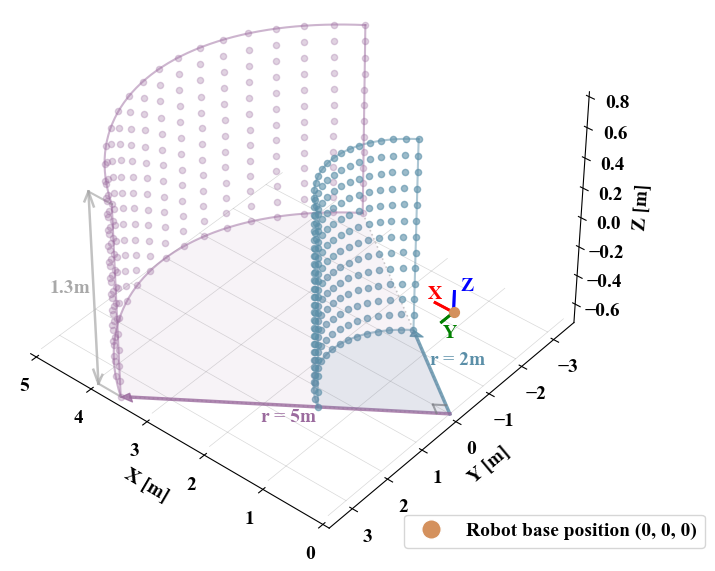
\includegraphics[width=0.9\columnwidth]{figure/adaptive_radius_3d.png}
    \caption{Illustration of the adaptive \RevisionAdd{sensing }radius mechanism \RevisionAdd{for the vertical distance map}. The vertical distance map is constructed on a cylindrical sector with a fixed number of cells ($17 \times 13$). A smaller radius (blue) provides higher spatial resolution for precise near-field sensing, while a larger radius (purple) extends the perception range at the cost of reduced resolution.
    The policy learns to dynamically adjust this radius based on the robot's locomotion state.}
    \label{fig:adaptive_radius}
\end{figure}

\subsubsection{Reward Functions}

The reward function $\mathcal{R}$ integrates multiple objectives to encourage robust and efficient locomotion adhering to safety constraints. The total reward \RevisionAdd{$\mathcal{R}_t = \sum_i w_i r_i(t)$ }is a weighted sum of the following components:

\begin{itemize}
    \item \textit{Motion Control:} Precise velocity tracking, postural stability, and energy efficiency are promoted by penalizing deviations in base orientation, excessive joint velocities or accelerations, and high-frequency action oscillations.

    \item \textit{Safety Mechanisms:} Safe and prolonged operation is ensured by penalizing critical failures such as body collisions, mesh interpenetrations, and joint limit violations. Furthermore, survival bonuses and foot air-time rewards are provided to foster dynamic and robust obstacle clearance.

    \item \textit{Active Perception:} \RevisionAdd{The sensing radius of the vertical distance map is learned jointly with locomotion through task rewards and two radius regularization terms. Their weighted contributions to the total reward are
    \[
    \begin{aligned}
    R_{\mathrm{smooth}}(t)&=-\lambda_s|r_t-r_{t-1}|,\\
    R_{\mathrm{reg}}(t)&=-\lambda_r(r_t-r_{\mathrm{init}})^2,
    \end{aligned}
    \]
    where $r_t$, $r_{t-1}$, and $r_{\mathrm{init}}$ denote the current, previous, and initial sensing radii. These terms discourage abrupt radius changes and deviations from the initial radius.}.
\end{itemize}

\subsubsection{Terrain Design}
\textit{BarrierTrack} (Fig.~\ref{fig:terrain}), a customized environment assembling discrete obstacle modules, is designed to cultivate versatile locomotion. Each episode features a sequence of five obstacles of the same terrain type with progressively increasing difficulty according to a curriculum schedule. 

A curriculum-based strategy is adopted where each terrain type $\tau$ is parameterized by a difficulty scalar $s \in [0, 1]$, and its generation parameters are interpolated as $\mathbf{p}_\tau(s) = (1-s)\,\mathbf{p}_\tau^{\min} + s\,\mathbf{p}_\tau^{\max}$ based on Table~\ref{tab:terrain_params}. Perlin noise is superimposed onto ground surfaces to simulate terrain irregularity and prevent overfitting.


\begin{figure}[t]
    \centering
    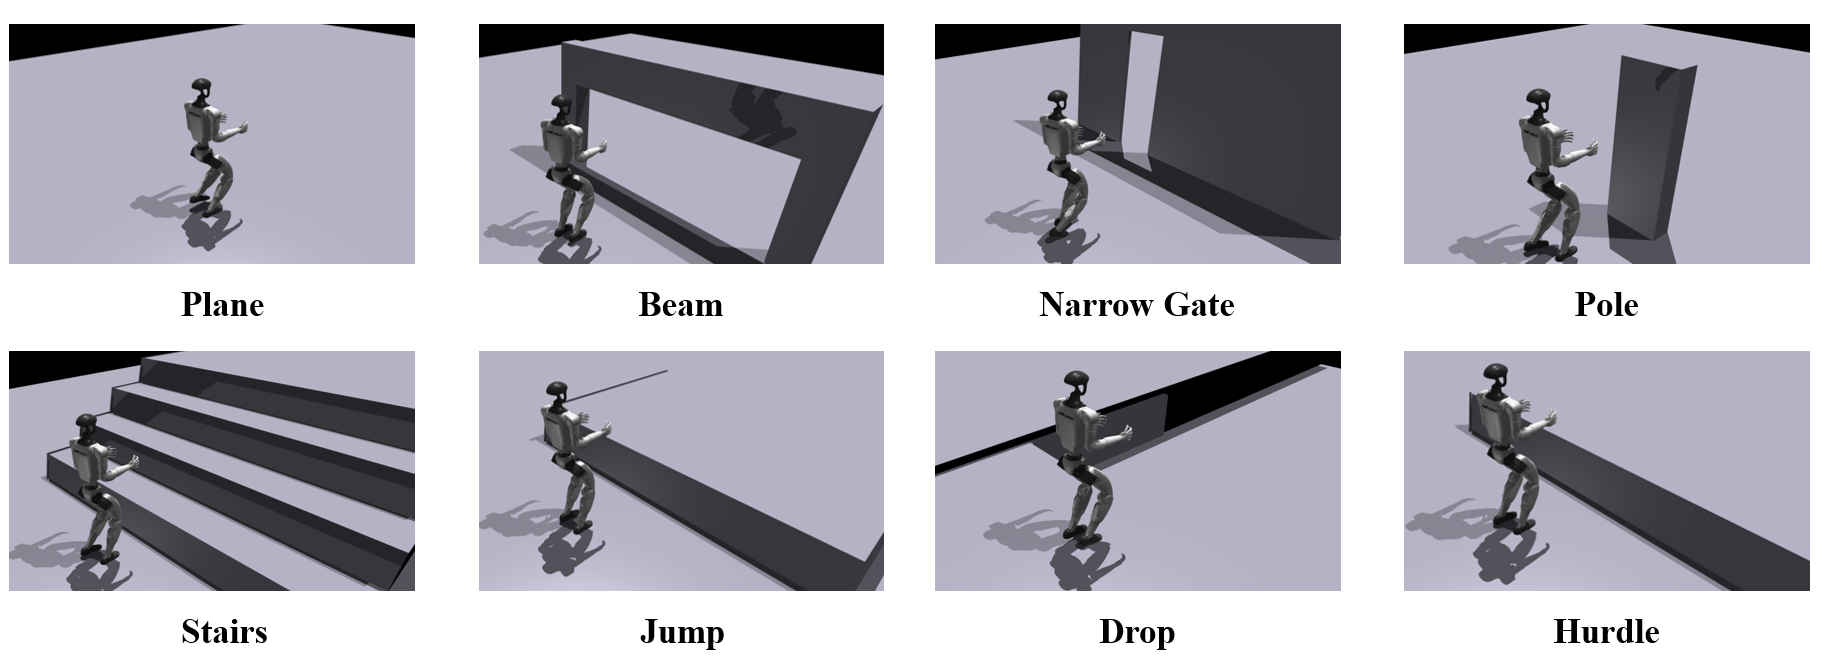
\includegraphics[width=\columnwidth]{figure/terrain.png}
    \caption{Examples of procedurally generated obstacles in our \textit{BarrierTrack} training environment. The curriculum includes a diverse set of challenges such as stairs, drop, hurdles, and constrained passages like beams and narrow gates, promoting the development of a versatile locomotion policy.}
    \label{fig:terrain}
\end{figure}

\subsection{Training Architecture}
\label{sec:training_architecture}

As shown in Fig.~\ref{fig:network_architecture}, two separate MLP encoders \RevisionAdd{map }$\mathbf{E}_t$ and $\mathbf{D}_t$ \RevisionAdd{to }32-dimensional \RevisionAdd{features, concatenated into }a 64-dimensional environmental embedding and fused with \RevisionAdd{proprioception before separate }actor and critic \RevisionAdd{LSTMs. The critic additionally receives the noise-free simulation elevation map; the actor uses only deployable observations}. \RevisionAdd{Let $\mathbf{h}_t^a$ and $\mathbf{h}_t^c$ denote the LSTM hidden states of the actor and critic at time step $t$, respectively. The recurrent inputs are $(\mathbf{h}_{t-1}^a,\mathbf{c}_{t-1}^a)$ for the actor and $(\mathbf{h}_{t-1}^c,\mathbf{c}_{t-1}^c)$ for the critic, where $\mathbf{c}_{t-1}^a$ and $\mathbf{c}_{t-1}^c$ denote their respective LSTM cell states at the previous time step. The actor's MLP maps $\mathbf{h}_t^a$ to joint targets and the next vertical-map sensing radius, closing the perception-control loop.}

% to effectively treat perception as an actuated degree of freedom.


%%%%%%%%%%%%%%%%%%%%%%%%%%%%%%%%%%%%%%%%%%%%%%%%%%%%%%%%%%%%%%%%%%%%%%%%%%%%%%%%
\section{Experiments}
\label{sec:experiment}

\subsection{Experimental Configuration}
\label{sec:method_terrain}

\subsubsection{Simulation Environment} 

\RevisionAdd{All policies are trained for a 12-DoF Unitree G1 humanoid robot using NVIDIA Isaac Gym~\cite{Isaac_Gym} on a modified NVIDIA RTX 4090 GPU with 48 GB of VRAM.} LiDAR point clouds are synthesized using the simulator from~\cite{Wang_2025_Omni-Perception} \RevisionAdd{to} accurately model sensor noises and occlusion from static terrains and dynamic robot links.

\subsubsection{Real-world Environment} The trained policy is then deployed on a physical Unitree G1 robot. A Livox Mid-360 LiDAR is mounted on the head to provide raw point cloud data. State estimation and point cloud registration are handled by Fast-LIO2~\cite{Xu_2022_FAST-LIO2}. \RevisionAdd{The horizontal elevation map }$\mathbf{E}_t$ \RevisionAdd{and the vertical distance map $\mathbf{D}_t$ }are extracted from the registered point cloud using the GPU-accelerated pipeline from~\cite{ElevationMap_GPU_2022} at $10$ Hz. 
% The vertical distance map $\mathbf{D}_t$ is generated at $10$ Hz as well. Registered points are projected into a polar sector spanning $-45^\circ$ to $+45^\circ$. Each map cell records the distance to the nearest obstacle. 
The map generation follows the exact same procedure used in simulation. \RevisionAdd{In all real-world deployment experiments, perception and policy inference run on a local computer with an Intel i7-12700H CPU and an NVIDIA RTX 3060 Laptop GPU with 6 GiB VRAM. The local computer generates and sends joint-angle targets to the robot at $50$ Hz}.

\subsection{Simulation Experiments}
\subsubsection{Evaluation Setup}
All methods are evaluated on the highest difficulty tier of \textit{BarrierTrack}. The benchmark includes all seven terrain primitives, grouped into two categories: terrains that require precise foot placement like Stairs, Drop, Jump and Hurdle, and the others that require traversable-space selection like Beam, Pole and Narrow Gate. For each terrain type, every episode contains five obstacles of the same class with progressively increasing difficulty; obstacle parameters are sampled within the range given in Table~\ref{tab:terrain_params} according to the curriculum schedule.

\begin{table}[t]
\vspace{3pt}
\centering
\caption{Parameters for generating curriculum training terrains. The $\uparrow$ symbol indicates the parameter value increases as difficulty scales up ($\mathbf{p}_\tau^{\min} < \mathbf{p}_\tau^{\max}$), while the $\downarrow$ symbol indicates the value decreases as the task becomes harder ($\mathbf{p}_\tau^{\min} > \mathbf{p}_\tau^{\max}$).}
\label{tab:terrain_params}
\setlength{\tabcolsep}{4pt}
\begin{tabular}{@{}llcc@{}}
\toprule
\textbf{Terrain} & \textbf{Param. (m)} & $\mathbf{p}_\tau^{\min}$ & $\mathbf{p}_\tau^{\max}$ \\
\midrule
\multirow{2}{*}{\textbf{Beam}} & Clearance Height $\downarrow$ & 1.33 & 1.10 \\
& Beam Depth $\uparrow$ & 0.20 & 0.20 \\
\addlinespace
\multirow{2}{*}{\textbf{Narrow Gate}} & Gate Width $\downarrow$ & 0.80 & 0.45 \\
& Position Offset $\uparrow$ & 0.00 & 0.60 \\
\addlinespace
\multirow{2}{*}{\textbf{Pole}} & Pole Width $\downarrow$ & 0.50 & 0.10 \\
& Position Offset $\uparrow$ & 0.00 & 0.00 \\
\addlinespace
\multirow{2}{*}{\textbf{Stairs}} & Step Height $\uparrow$ & 0.10 & 0.30 \\
& Step Length $\downarrow$ & 0.50 & 0.30 \\
\addlinespace
\multirow{2}{*}{\textbf{Jump}} & Wall Height $\uparrow$ & 0.05 & 0.40 \\
& Wall Depth $\uparrow$ & 0.10 & 0.30 \\
\addlinespace
\multirow{2}{*}{\textbf{Drop}} & Drop Height $\uparrow$ & 0.10 & 0.60 \\
& Platform Length $\downarrow$ & 0.50 & 0.30 \\
\addlinespace
\multirow{2}{*}{\textbf{Hurdle}} & Hurdle Height $\uparrow$ & 0.05 & 0.40 \\
& Hurdle Depth $\uparrow$ & 0.05 & 0.10 \\
\bottomrule
\end{tabular}
\end{table}

\subsubsection{Metrics}
Robot performance is evaluated by the mean and standard deviations over two metrics:
(1) Success Rate ($R_{\mathrm{succ}}$), which is the fraction of discrete obstacles that the robot successfully navigates within a single trial, i.e., the number of obstacles crossed divided by 5, 
% It measures the policy's obstacle-negotiation reliability.
and (2) Normalized Traversal Progress ($R_{\mathrm{trav}}$), which is the forward distance traveled along the course normalized by the total track length. Note that $R_{\mathrm{trav}}$ is typically no lower than $R_{\mathrm{succ}}$, as the robot may stumble forward for some distance even after failing to clear an obstacle, thereby accumulating partial traversal progress.
% It evaluates the overall capability to string together continuous locomotion skills.

\subsubsection{Performance Comparison}
ADAPT is benchmarked against four baselines to evaluate its navigation capability and computational efficiency.
Each method is evaluated across all seven terrain types under three speed commands: $v \in \{0.5, 1.0, 1.5\}$\,m/s.
For each terrain-speed combination, 10 trials are conducted and the average results are reported.
The four selected baselines are:
\begin{itemize}
    \item PIM~\cite{long2025learning}: A single-stage training method that uses an elevation map from LiDAR point cloud as exteroceptive input. Contrastive learning aligns the generated elevation map with ground truth.
    \item Parkour~\cite{zhuang2024humanoid}: A two-stage method where a teacher policy is first trained with ground-truth elevation maps and then agile locomotion skills are transferred through supervised distillation to a student policy that only uses depth images.
    \item TSDF: A camera-based approach that performs 3D reconstruction via nvblox~\cite{nvblox_2023_GPUAcceleratedSDFMapping} and feeds local grid TSDF values as exteroceptive input for policy training.
    \item Gallant~\cite{Ben_2025_Gallant}: A voxel-based approach that provides full 3D awareness but at a higher computational cost.
\end{itemize}

\begin{table*}[t]
\vspace{3pt}
\centering
\caption{Benchmarked Comparison in Simulation. $R_\mathrm{succ}$: success rate (\%, $\uparrow$). $R_\mathrm{trav}$: normalized traversal progress (\%, $\uparrow$).}
\label{tab:main_results}
\setlength{\tabcolsep}{4pt}
% \begin{center}
\begin{tabular}{lcccccccc}
\toprule[1.0pt]
\multirow{2}{*}{Method} &
\multicolumn{2}{c}{Plane} & \multicolumn{2}{c}{Stairs} & \multicolumn{2}{c}{Drop} & \multicolumn{2}{c}{Jump} \\
\cmidrule(lr){2-3}\cmidrule(lr){4-5}\cmidrule(lr){6-7}\cmidrule(lr){8-9}
& $R_\mathrm{succ}$ & $R_\mathrm{trav}$ & $R_\mathrm{succ}$ & $R_\mathrm{trav}$ & $R_\mathrm{succ}$ & $R_\mathrm{trav}$ & $R_\mathrm{succ}$ & $R_\mathrm{trav}$ \\
\midrule[0.8pt]
PIM~\cite{long2025learning}        & 100\ci{0.0} & 100\ci{0.0} & 65.33\ci{37.57} & 70.00\ci{34.61} & 99.33\ci{3.59} & 99.77\ci{1.26} & 90.67\ci{16.92} & 91.67\ci{14.62} \\[0.4ex]
Parkour~\cite{zhuang2024humanoid}  & 100\ci{0.0} & 100\ci{0.0} & 28.00\ci{28.10} & 37.20\ci{24.93} & 91.33\ci{14.31} & 92.40\ci{13.52} & 44.67\ci{20.45} & 51.40\ci{17.49} \\[0.4ex]
TSDF                               & 100\ci{0.0} & 100\ci{0.0} & 40.00\ci{20.00} & 47.43\ci{17.50} & 56.67\ci{24.81} & 63.33\ci{22.75} & 43.33\ci{13.74} & 48.63\ci{13.65} \\[0.4ex]
Gallant~\cite{Ben_2025_Gallant}    & 100\ci{0.0} & 100\ci{0.0} & 70.00\ci{22.95} & 76.30\ci{21.75} & 80.00\ci{31.41} & 83.23\ci{27.62} & 68.00\ci{13.27} & 74.10\ci{11.34} \\[0.4ex]
\textbf{Ours}                      & \textbf{100\ci{0.0}} & \textbf{100\ci{0.0}} & \textbf{94.67\ci{13.60}} & \textbf{95.90\ci{10.63}} & \textbf{100.00\ci{0.00}} & \textbf{100.00\ci{0.00}} & \textbf{98.67\ci{4.99}} & \textbf{98.90\ci{4.12}} \\[0.4ex]
\midrule[0.8pt]
\multirow{2}{*}{Method} &
\multicolumn{2}{c}{Hurdle} & \multicolumn{2}{c}{Beam} & \multicolumn{2}{c}{Pole} & \multicolumn{2}{c}{Narrow Gate} \\
\cmidrule(lr){2-3}\cmidrule(lr){4-5}\cmidrule(lr){6-7}\cmidrule(lr){8-9}
& $R_\mathrm{succ}$ & $R_\mathrm{trav}$ & $R_\mathrm{succ}$ & $R_\mathrm{trav}$ & $R_\mathrm{succ}$ & $R_\mathrm{trav}$ & $R_\mathrm{succ}$ & $R_\mathrm{trav}$ \\
\midrule[0.4pt]
PIM~\cite{long2025learning}        & 82.00\ci{20.88} & 86.37\ci{16.44} & 66.67\ci{9.43} & 75.53\ci{5.28} & 2.67\ci{6.80} & 6.17\ci{7.09} & 27.33\ci{15.04} & 31.17\ci{14.17} \\[0.4ex]
Parkour~\cite{zhuang2024humanoid}  & 47.33\ci{13.15} & 52.67\ci{12.81} & 14.00\ci{11.72} & 20.53\ci{6.93} & 5.33\ci{8.84} & 15.00\ci{7.90} & 48.00\ci{16.81} & 53.03\ci{16.05} \\[0.4ex]
TSDF                               & 49.33\ci{11.23} & 55.47\ci{13.98} & 33.33\ci{11.93} & 40.83\ci{11.37} & 7.33\ci{9.64} & 14.37\ci{9.07} & 22.67\ci{16.11} & 29.80\ci{14.31} \\[0.4ex]
Gallant~\cite{Ben_2025_Gallant}    & 54.67\ci{16.28} & 62.47\ci{14.21} & 32.00\ci{25.61} & 40.40\ci{27.17} & 46.00\ci{44.17} & 49.40\ci{41.82} & 66.00\ci{25.90} & 69.57\ci{23.35} \\[0.4ex]
\textbf{Ours}                      & \textbf{90.00\ci{14.38}} & \textbf{91.80\ci{12.80}} & \textbf{96.67\ci{7.45}} & \textbf{97.57\ci{5.47}} & \textbf{98.00\ci{6.00}} & \textbf{98.57\ci{4.79}} & \textbf{80.00\ci{18.62}} & \textbf{83.03\ci{16.30}} \\[0.4ex]
\bottomrule[1.0pt]
\end{tabular}
% \end{center}
\end{table*}

\RevisionAdd{Table~\ref{tab:main_results} details the performance comparison}.
% , while Table~\ref{tab:efficiency}\RevisionAdd{(a) }presents the associated training costs. 
ADAPT (Ours) achieves the highest success rates across all terrains while requiring \RevisionAdd{less training time per iteration and lower peak GPU memory than the Gallant and TSDF baselines}.
The performance of the baselines is consistent with the sensing characteristics within each method.
PIM relies on a 2.5D elevation map and shows reduced performance on Pole and Narrow Gate terrains where vertical and lateral clearance cues are important. Parkour uses depth images and performs less reliably on terrains requiring broader spatial coverage, such as Jump, Hurdle and Beam. TSDF provides volumetric awareness, but its performance remains limited on fine-grained terrains although incurring the highest training cost. Gallant improves spatial coverage relative to the other baselines, but its higher-dimensional voxel input requires higher computational cost and achieves lower success rates than ADAPT on most terrains. Overall, ADAPT provides a favorable balance between traversal performance and computation efficiency across various tasks.

\RevisionAdd{Although voxels preserve richer 3D geometry, our Gallant implementation trades sensing coverage for fine resolution under a fixed voxel count and computational budget. Its performance gap widens at high speeds, where obstacles entering view trigger abrupt deceleration and occasional imbalance, suggesting insufficient look-ahead for smooth motion adjustment. ADAPT instead adjusts its look-ahead distance to the robot's motion state.
}

\RevisionAdd{All methods use identical hardware and training settings (parallel environments, rollout length, PPO epochs, and batch settings). Table~\ref{table:comparison_method} compares per-frame, pre-encoding actor exteroceptive dimensions: Gallant uses $32\times32\times40=40{,}960$ values and ADAPT uses $21\times17+13\times17=578$, a $98.6\%$ reduction. Proprioception, observation history, and critic-only inputs are excluded.
Table~\ref{tab:efficiency}(a) reports wall-clock iteration time and peak single-GPU memory monitored with \texttt{nvidia-smi}. Relative to Gallant, ADAPT reduces iteration time from $34.6$ to $11.3$ s ($32.7\%$ of the baseline) and peak memory from $36{,}054$ to $15{,}870$ MiB ($56.0\%$ lower).
}

\begin{table*}[t]
\centering
\caption{Training \RevisionAdd{and Runtime }Efficiency. \RevisionAdd{Runtime latencies}: \RevisionAdd{averages of per-trial means/P95s }(\RevisionAdd{ms}). \RevisionAdd{ADAPT reports the larger of the two map-stream statistics for each map-latency and perception-to-publish latency entry}. \RevisionAdd{Resources: mean whole-host CPU utilization}/\RevisionAdd{RAM usage and maximum sampled VRAM usage}.}
\label{tab:efficiency}
\small
\setlength{\tabcolsep}{6pt}
\RevisionAdd{\textbf{(a) Training efficiency}}\\[3pt]
\begin{tabular}{lcc}
\toprule[1.0pt]
Method & Train/iter (s) & \RevisionAdd{Peak VRAM (MiB}) \\
\midrule[0.8pt]
PIM~\cite{long2025learning} & 2.6 & 10485 \\
Parkour~\cite{zhuang2024humanoid} & 97.8 & 28791 \\
Gallant~\cite{Ben_2025_Gallant} & 34.6 & 36054 \\
TSDF & 246 & 38473 \\
\textbf{\RevisionAdd{ADAPT (}Ours\RevisionAdd{)}} & \textbf{11.3} & \textbf{15870} \\
\bottomrule[1.0pt]
\end{tabular}
\par\vspace{6pt}
\RevisionAdd{\textbf{(b) Local-computer runtime latency and resource usage}}\\[3pt]
\setlength{\tabcolsep}{4pt}
\begin{tabular}{lccccc}
\toprule[1.0pt]
\RevisionAdd{Method }& \RevisionAdd{Map latency }& \RevisionAdd{Inference latency }& \RevisionAdd{Perception-to-publish latency }& \RevisionAdd{Peak VRAM }& \RevisionAdd{CPU / RAM }\\
 & \RevisionAdd{Mean/P95 (ms) }& \RevisionAdd{Mean/P95 (ms) }& \RevisionAdd{Mean/P95 (ms) }& \RevisionAdd{(MiB) }& \RevisionAdd{(\% / GiB) }\\
\midrule[0.8pt]
\RevisionAdd{Gallant }& \RevisionAdd{64.06 / 87.49 }& \RevisionAdd{1.91 / 3.20 }& \RevisionAdd{79.45 / 106.09 }& \RevisionAdd{5711 }& \RevisionAdd{38.19 / 10.66 }\\
\RevisionAdd{ADAPT }& \RevisionAdd{\textbf{41.64 / 64.09} }& \RevisionAdd{\textbf{1.40 / 1.96} }& \RevisionAdd{\textbf{55.94 / 79.31} }& \RevisionAdd{\textbf{2373} }& \RevisionAdd{\textbf{17.76 / 8.04} }\\
\bottomrule[1.0pt]
\end{tabular}
\end{table*}


\RevisionAdd{Besides, although PIM has the lowest training cost, it lacks body-clearance information. ADAPT incurs a moderate cost increase over PIM while remaining cheaper than the volumetric baselines}.

\subsubsection{Ablation Study on Adaptive Mechanism}
To specifically validate the obstacle avoidance capability of the adaptive mechanism, the ablation study focuses on Beam, Pole and Narrow Gate terrains where perception is critical. \RevisionAdd{For each method, terrain, and speed command, 10 trials are conducted in simulation. 
% Table~\ref{tab:ablation_radius} reports the success rate averaged over the three terrains.
}

Besides the proposed method, two additional settings isolating the effect of radius representation and reward formulation are considered:
1) \textit{Fixed Radius}, where the sensing radius $r_t$ is excluded from the observation and action spaces. The policy operates with a constant radius. Separate policies are trained with $R \in \{1, 3, 5\}$\,m.
2) \textit{w/o Adaptive Reward}, where $r_t$ \RevisionAdd{remains }both an observation and an action, \RevisionAdd{but the radius smoothness term $R_{\mathrm{smooth}}(t)$
and radius regularization term $R_{\mathrm{reg}}(t)$ are removed. All other reward terms are retained}.

Table~\ref{tab:ablation_radius} summarizes the ablation results. \RevisionAdd{As in the main benchmark, each trial evaluates traversal through a sequence of five obstacles of the same terrain type at a fixed speed command. The success rate $R_{\mathrm{succ}}$ is the fraction of the five obstacles being successfully crossed in a trial. The table reports the mean and standard deviation over the 30 trial-level success rates pooled across Beam, Pole, and Narrow Gate at each speed}.

A short fixed radius ($R=1$) yields the lowest average success rates, particularly at higher speeds, indicating that the limited look-ahead range is insufficient for these terrains. 
% A long fixed radius ($R=5$) performs better than $R=1$ at high speed but remains clearly below the full adaptive model, suggesting a trade-off between larger look-ahead range and reduced local resolution. A moderate fixed radius ($R=3$) outperforms both extremes, but its performance still drops as commanded speed increases. This drop can be further enlarged at $v=1.5$\,m/s if the adaptive reward is fully removed (w/o Adaptive Reward), which indicates that treating the sensing radius as an action alone is not sufficient to recover the best sensing behavior. 
A long fixed radius ($R=5$) performs better than $R=1$ at high speeds but remains inferior to a moderate fixed radius ($R=3$), suggesting a trade-off between larger look-ahead range and reduced local resolution. However, the performance of a fixed radius is still behind the fully adaptive method. \RevisionAdd{Removing both radius-related rewards in \textit{w/o Adaptive Reward} lowers success at higher speeds, where less time for perception and avoidance may increase sensitivity to unsuitable or fluctuating sensing ranges. Together, the smoothness and regularization terms help stabilize radius selection and its coordination with locomotion}.
Overall, the fully adaptive method achieves the highest average success rate, indicating efficacy of the proposed closed-loop radius modulation.

\begin{table}[t]
\centering
\caption{Ablation on adaptive sensing radius. $R_\mathrm{succ}$: success rate (\%). Values are averaged over Beam, Pole, and Narrow Gate terrains.}
\label{tab:ablation_radius}
\begin{center}
\resizebox{\columnwidth}{!}{%
\begin{tabular}{llccc}
\toprule[1.0pt]
Type & Config & $v{=}0.5$\,m/s & $v{=}1.0$\,m/s & $v{=}1.5$\,m/s \\
\midrule[0.8pt]
\multirow{3}{*}{Fixed Radius}  & $R = 1$               & 51.33\ci{17.65} & 51.33\ci{23.49} & 24.67\ci{22.32} \\[0.4ex]
                               & $R = 3$               & 81.33\ci{21.25} & 72.67\ci{15.90} & 56.67\ci{29.70} \\[0.4ex]
                               & $R = 5$               & 64.00\ci{18.90} & 64.67\ci{26.17} & 53.33\ci{30.26} \\
\midrule[0.5pt]
w/o Adap.\ Reward              & no $r_{\text{adapt}}$  & 92.67\ci{10.93} & 71.33\ci{25.66} & 42.67\ci{29.09} \\
\midrule[0.5pt]
Adaptive Radius                & \textbf{Ours}         & \textbf{94.67\ci{10.24}} & \textbf{96.00\ci{8.00}} & \textbf{84.00\ci{19.60}} \\
\bottomrule[1.0pt]
\end{tabular}%
}
\end{center}
\end{table}

\begin{figure*}[t]
    \centering
    \includegraphics[width=0.8\linewidth]{figure/real_deploy.png}
    \caption{Zero-shot real-world deployment across diverse terrains. The trained policy enables the physical robot to successfully traverse seven distinct \textit{BarrierTrack} terrains without any real-world fine-tuning.}
    \label{fig:real_deploy}
\end{figure*}

\subsection{Real-world Experiments}
\subsubsection{Deployment}

\RevisionAdd{ADAPT transfers directly to the Unitree G1 without fine-tuning (Fig.~\ref{fig:real_deploy}). In Fig.~\ref{fig:succ}, final checkpoints from ten independent training seeds are evaluated in matched simulation and real-world scenes with a fixed single-obstacle configuration per terrain. Each policy is tested once per terrain at each speed ($v\in\{0.5,1.0,1.5\}$\,m/s), totaling 30 trials per terrain and domain}.

In terrains that require traversable-space selection, the robot identifies viable regions using the vertical distance map $\mathbf{D}_t$. When encountering aerial obstacles such as beams, the robot lowers its body to crouch underneath the beams and resumes to the normal posture afterward. For narrow pillar-like obstacles, the robot autonomously adjusts its heading to bypass the poles. When facing narrow gates, it precisely aligns its orientation with the traversable path. In terrains requiring precise foot placement, the robot relies on the elevation map $\mathbf{E}_t$ to stably ascend stairs, negotiate drops and jumps, and step over hurdles. \RevisionAdd{The adaptive sensing radius of the vertical distance map further enables the policy to regulate its perception horizon online during high-speed locomotion}.

\subsubsection{Results}

\begin{figure}[t]
\captionsetup{textfont={color=red},labelfont={color=red}}
    \centering
    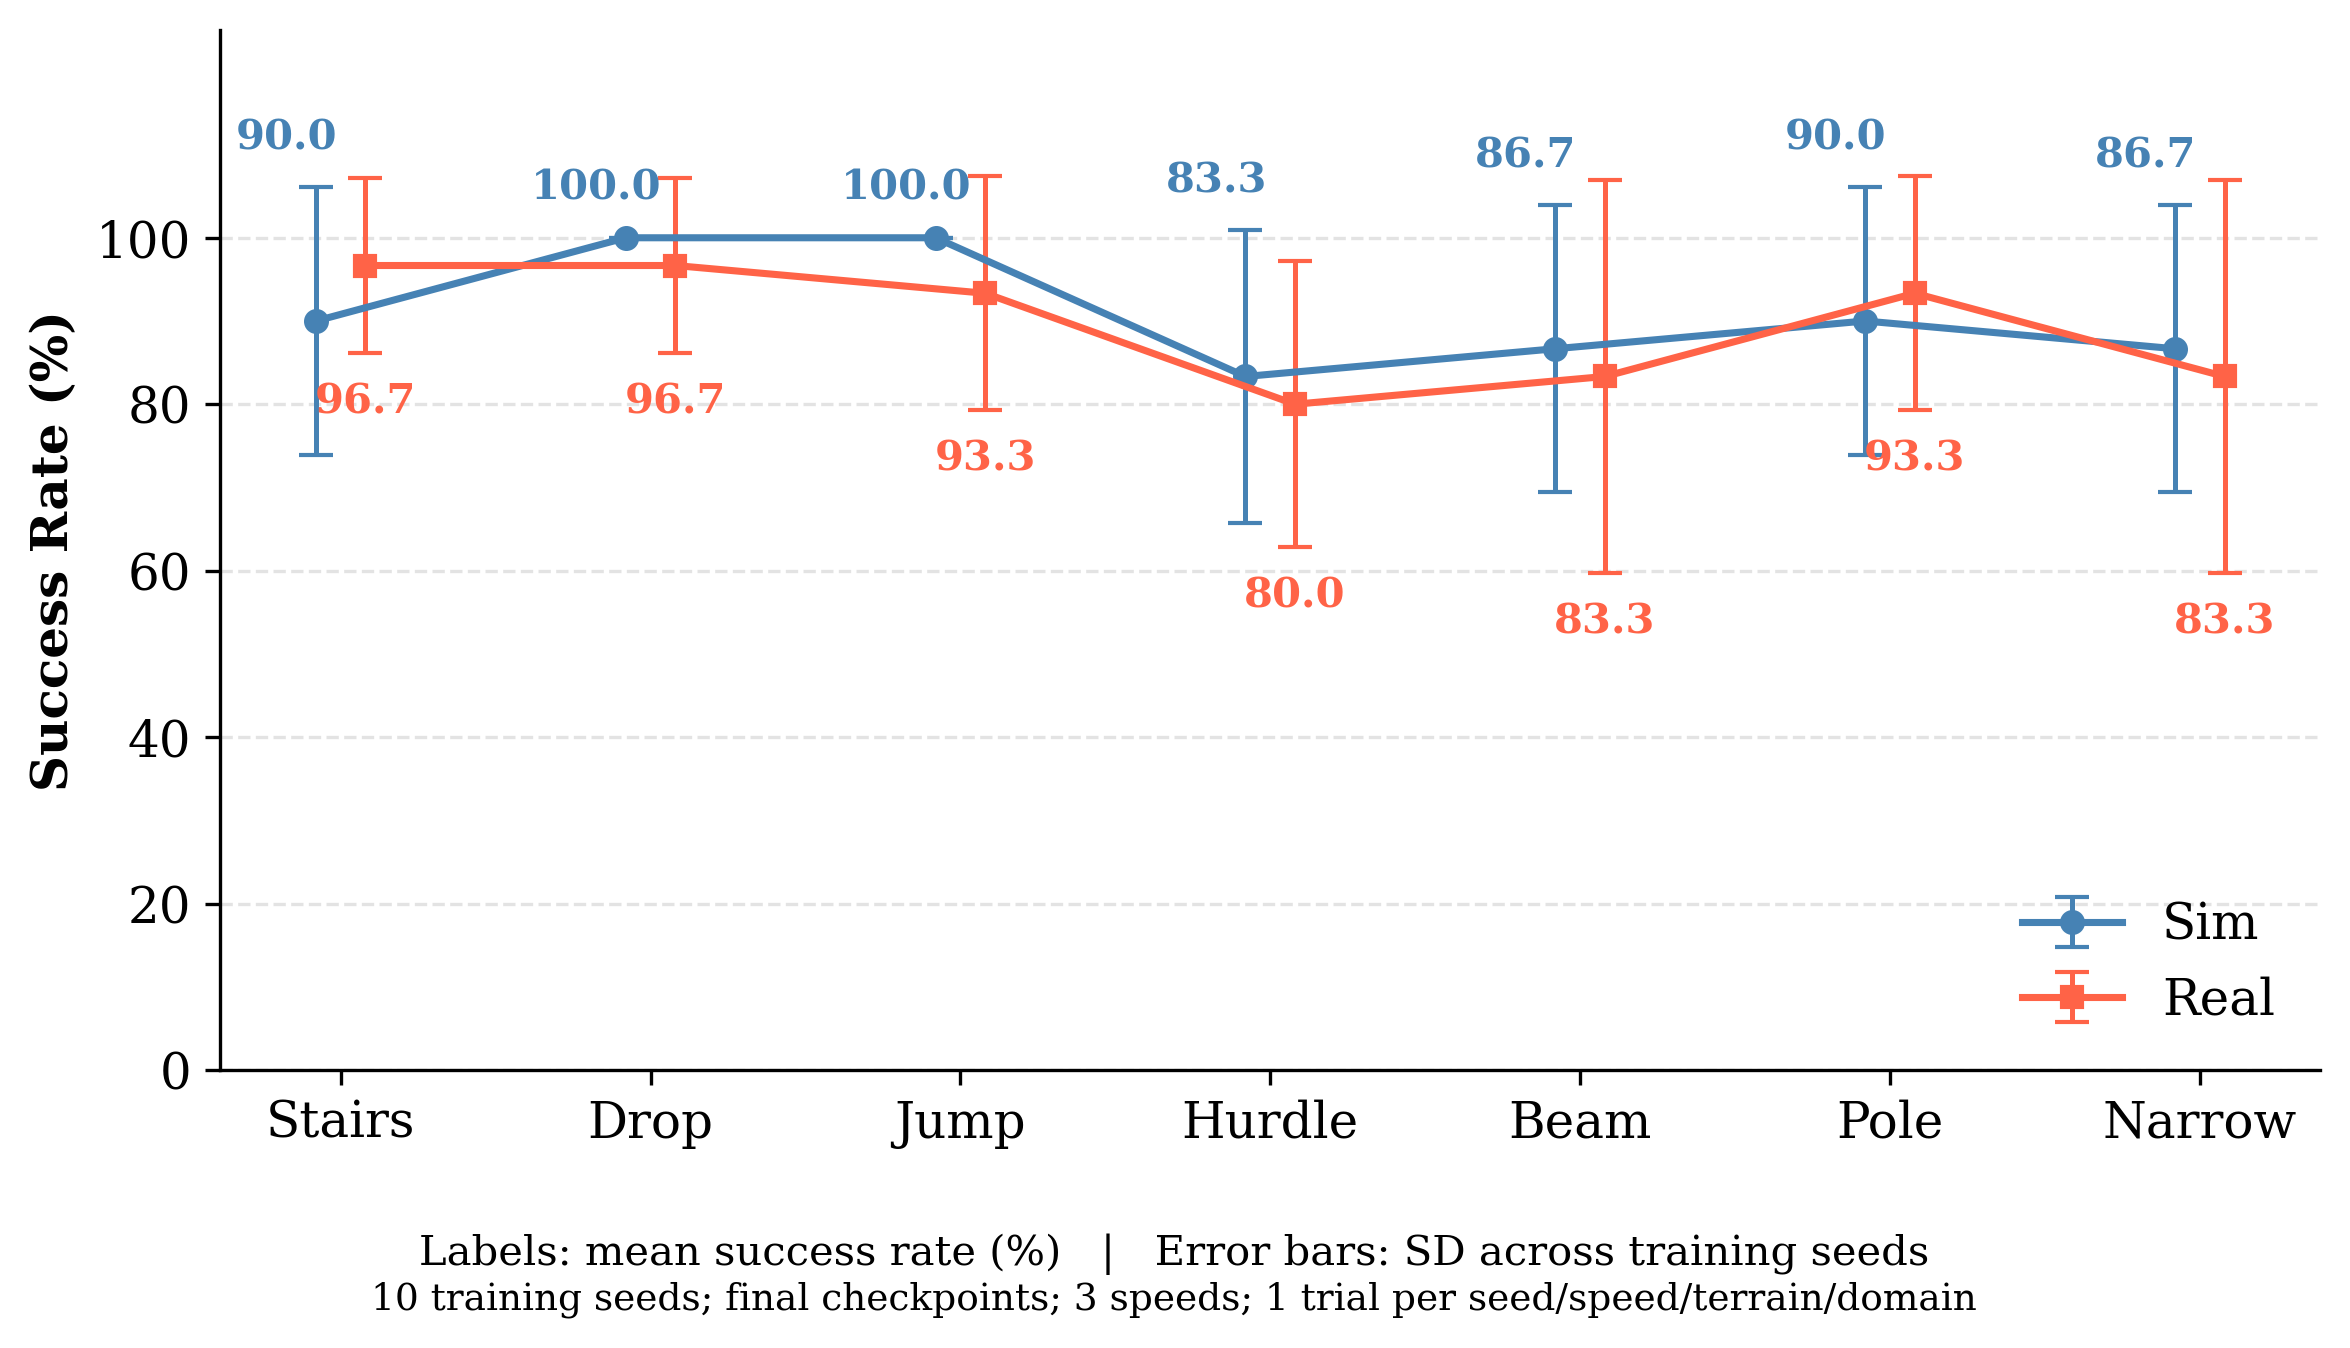
\includegraphics[width=0.9\linewidth]{figure/success_rate_sim_real.png}
    \caption{\RevisionAdd{Single-obstacle traversal success }rates in \RevisionAdd{matched }simulation and real-world \RevisionAdd{scenes}. \RevisionAdd{Points and error bars show the mean and sample standard deviation across ten training seeds, after averaging }each \RevisionAdd{policy's outcomes }over \RevisionAdd{three speeds}.}
    \label{fig:succ}
    % \vspace{-5pt}
\end{figure}

\RevisionAdd{As a result, Fig.~\ref{fig:real_deploy} demonstrates zero-shot sim-to-real transfer across all seven terrains, while Fig.~\ref{fig:succ} presents the corresponding per-terrain success rates in simulation and physical deployment.} Despite an inherent sim-to-real domain gap, the real-world success rates closely follow the trend of their counterparts in simulation, maintaining \RevisionAdd{at least }$80\%$ success rates across all terrains. The physical robot exhibits a range of whole-body behaviors, including stair ascent and descent, stepping across drops and gaps, crouching under beams of varying height, and navigating through narrow passages and pole fields, suggesting good generality and practical applicability of the learned policy. 

\subsubsection{\RevisionAdd{Runtime Efficiency}}
\RevisionAdd{Table~\ref{tab:efficiency}(b) compares ADAPT and Gallant on a local computer (i7-12700H, RTX 3060 Laptop GPU with 6 GiB VRAM). The runtime benchmarks use the same local-computer deployment setup as the real-world robot experiments. Each method is tested five times on each of three terrain categories (flat, single obstacle, and complex environment). Map latency spans the input callback to the first observed map-ready event; perception-to-publish latency spans the same input callback to the first command-publication call using that update. Inference latency is measured using current-stream CUDA events. ADAPT reduces mean perception-to-publish latency by $29.6\%$ using the larger of the two stream means and peak GPU memory by $58.4\%$ relative to Gallant, with lower CPU/RAM usage.
}

% \subsection{Discussion}

% The consistent sim-to-real performance confirms that ADAPT's two design choices—the vertical distance map for compact 3D constraint encoding and the adaptive sensing radius for online horizon regulation—are more effective than heavy 3D reconstruction or multi-stage training. Well-structured inputs matter more than model complexity for agile humanoid navigation.

\section{Conclusions}
This paper presents ADAPT, an adaptive dual-projection framework for perceptive humanoid traversal in complex 3D environments. By decomposing local geometry into a horizontal elevation map and a vertical distance map, ADAPT explicitly separates ground-support and body-level clearance constraints into a compact representation for high-frequency control. Furthermore, embedding the sensing radius into the action space enables the robot to dynamically adjust its perceptual horizon based on motion context. Experiments demonstrate that ADAPT significantly improves traversal robustness and computational efficiency over fixed-range and voxel-based alternatives, achieving successful zero-shot sim-to-real transfer on a Unitree G1 robot.

Despite these capabilities, the current framework focuses solely on geometric traversability and adapts only the sensing radius. Future work will investigate richer active perception policies that jointly optimize sensing scale, resolution, and update frequency, while incorporating semantic reasoning to enable long-horizon navigation in complex, human-centered environments.

%%%%%%%%%%%%%%%%%%%%%%%%%%%%%%%%%%%%%%%%%%%%%%%%%%%%%%%%%%%%%%%%%%%%%%%%%%%%%%%%
% References
%%%%%%%%%%%%%%%%%%%%%%%%%%%%%%%%%%%%%%%%%%%%%%%%%%%%%%%%%%%%%%%%%%%%%%%%%%%%%%%%
%%%%%%%%%%%%%%%%%%%%%%%%%%%%%%%%%%%%%%%%%%%%%%%%%%%%%%%%%%%%%%%%%%%%%%%%%%%%%%%%
% References
%%%%%%%%%%%%%%%%%%%%%%%%%%%%%%%%%%%%%%%%%%%%%%%%%%%%%%%%%%%%%%%%%%%%%%%%%%%%%%%%
\balance

\begin{thebibliography}{10}
\providecommand{\url}[1]{#1}
\csname url@rmstyle\endcsname
\providecommand{\newblock}{\relax}
\providecommand{\bibinfo}[2]{#2}
\providecommand\BIBentrySTDinterwordspacing{\spaceskip=0pt\relax}
\providecommand\BIBentryALTinterwordstretchfactor{4}
\providecommand\BIBentryALTinterwordspacing{\spaceskip=\fontdimen2\font plus
\BIBentryALTinterwordstretchfactor\fontdimen3\font minus
  \fontdimen4\font\relax}
\providecommand\BIBforeignlanguage[2]{{%
\expandafter\ifx\csname l@#1\endcsname\relax
\typeout{** WARNING: IEEEtran.bst: No hyphenation pattern has been}%
\typeout{** loaded for the language `#1'. Using the pattern for}%
\typeout{** the default language instead.}%
\else
\language=\csname l@#1\endcsname
\fi
#2}}

\bibitem{Fankhauser2014RobotCentricElevationMapping}
P.~Fankhauser, M.~Bloesch, C.~Gehring, M.~Hutter, and R.~Siegwart,
  ``Robot-centric elevation mapping with uncertainty estimates,'' in
  \emph{International Conference on Climbing and Walking Robots (CLAWAR)},
  2014.

\bibitem{Fankhauser2018ProbabilisticTerrainMapping}
P.~Fankhauser, M.~Bloesch, and M.~Hutter, ``Probabilistic terrain mapping for
  mobile robots with uncertain localization,'' \emph{IEEE Robotics and
  Automation Letters (RA-L)}, vol.~3, no.~4, pp. 3019--3026, 2018.

\bibitem{ElevationMap_GPU_2022}
T.~{Miki}, L.~{Wellhausen}, R.~{Grandia}, F.~{Jenelten}, T.~{Homberger}, and
  M.~{Hutter}, ``{Elevation Mapping for Locomotion and Navigation using GPU},''
  \emph{arXiv e-prints}, p. arXiv:2204.12876, Apr. 2022.

\bibitem{long2025learning}
J.~Long, J.~Ren, M.~Shi, Z.~Wang, T.~Huang, P.~Luo, and J.~Pang, ``Learning
  humanoid locomotion with perceptive internal model,'' in \emph{2025 IEEE
  International Conference on Robotics and Automation (ICRA)}.\hskip 1em plus
  0.5em minus 0.4em\relax IEEE, 2025, pp. 9997--10\,003.

\bibitem{wang2025beamdojo}
H.~Wang, Z.~Wang, J.~Ren, Q.~Ben, T.~Huang, W.~Zhang, and J.~Pang, ``Beamdojo:
  Learning agile humanoid locomotion on sparse footholds,'' \emph{arXiv
  preprint arXiv:2502.10363}, 2025.

\bibitem{ren2025vb}
J.~Ren, T.~Huang, H.~Wang, Z.~Wang, Q.~Ben, J.~Long, Y.~Yang, J.~Pang, and
  P.~Luo, ``Vb-com: Learning vision-blind composite humanoid locomotion against
  deficient perception,'' \emph{arXiv preprint arXiv:2502.14814}, 2025.

\bibitem{he2025attention}
J.~He, C.~Zhang, F.~Jenelten, R.~Grandia, M.~B{\"a}cher, and M.~Hutter,
  ``Attention-based map encoding for learning generalized legged locomotion,''
  \emph{Science Robotics}, vol.~10, no. 105, p. eadv3604, 2025.

\bibitem{videomimic}
A.~Allshire, H.~Choi, J.~Zhang, D.~McAllister, A.~Zhang, C.~M. Kim, T.~Darrell,
  P.~Abbeel, J.~Malik, and A.~Kanazawa, ``Visual imitation enables contextual
  humanoid control,'' \emph{arXiv preprint arXiv:2505.03729}, 2025.

\bibitem{Multi-Layer_ElevationMap_2025}
Y.~{Chen}, J.~{Ma}, Z.~{Luo}, Y.~{Han}, Y.~{Dong}, B.~{Xu}, and P.~{Lu},
  ``{Learning Autonomous and Safe Quadruped Traversal of Complex Terrains Using
  Multi-Layer Elevation Maps},'' \emph{IEEE Robotics and Automation Letters},
  vol.~10, no.~10, pp. 9606--9613, Jan. 2025.

\bibitem{Roth_2025_LearnedPerceptiveForwardDynamicsModel}
P.~{Roth}, J.~{Frey}, C.~{Cadena}, and M.~{Hutter}, ``{Learned Perceptive
  Forward Dynamics Model for Safe and Platform-aware Robotic Navigation},''
  \emph{arXiv e-prints}, p. arXiv:2504.19322, Apr. 2025.

\bibitem{Zhang_2026_AME2}
C.~{Zhang}, V.~{Klemm}, F.~{Yang}, and M.~{Hutter}, ``{AME-2: Agile and
  Generalized Legged Locomotion via Attention-Based Neural Map Encoding},''
  \emph{arXiv e-prints}, p. arXiv:2601.08485, Jan. 2026.

\bibitem{Li_2024_MOVE}
S.~{Li}, S.~{Luo}, J.~{Wu}, and Q.~{Zhu}, ``{MOVE: Multi-skill Omnidirectional
  Legged Locomotion with Limited View in 3D Environments},'' \emph{arXiv
  e-prints}, p. arXiv:2412.03353, Dec. 2024.

\bibitem{zhuang2024humanoidRobot}
Z.~Zhuang, Z.~Fu, J.~Wang, C.~G. Atkeson, S.~Schwertfeger, C.~Finn, and
  H.~Zhao, ``Robot parkour learning,'' \emph{arXiv preprint arXiv:2309.05665},
  2024.

\bibitem{zhuang2024humanoid}
Z.~Zhuang, S.~Yao, and H.~Zhao, ``Humanoid parkour learning,'' \emph{arXiv
  preprint arXiv:2406.10759}, 2024.

\bibitem{Yu_2025_START}
R.~{Yu}, Q.~{Wang}, H.~{Li}, Z.~{Jun}, Z.~{Wang}, J.~{Wu}, and Q.~{Zhu},
  ``{START: Traversing Sparse Footholds with Terrain Reconstruction},''
  \emph{arXiv e-prints}, p. arXiv:2512.13153, Dec. 2025.

\bibitem{Castillo_2025_LearningTerrainAwareBipedalLocomotion}
G.~A. {Castillo}, H.~{Lodha}, and A.~{Hereid}, ``{Learning Terrain Aware
  Bipedal Locomotion via Reduced Dimensional Perceptual Representations},''
  \emph{arXiv e-prints}, p. arXiv:2512.12993, Dec. 2025.

\bibitem{Solano_2025_StandWalkNavigate}
J.~{Solano} and D.~{Quiroz}, ``{Stand, Walk, Navigate: Recovery-Aware Visual
  Navigation on a Low-Cost Wheeled Quadruped},'' \emph{arXiv e-prints}, p.
  arXiv:2510.23902, Oct. 2025.

\bibitem{Sun_2025_DPL}
J.~{Sun}, G.~{Han}, P.~{Sun}, W.~{Zhao}, J.~{Cao}, J.~{Wang}, Y.~{Guo}, and
  Q.~{Zhang}, ``{DPL: Depth-only Perceptive Humanoid Locomotion via Realistic
  Depth Synthesis and Cross-Attention Terrain Reconstruction},'' \emph{arXiv
  e-prints}, p. arXiv:2510.07152, Oct. 2025.

\bibitem{Wang_2025_LocoMamba}
Y.~{Wang} and G.~{Tao}, ``{LocoMamba: Vision-Driven Locomotion via End-to-End
  Deep Reinforcement Learning with Mamba},'' \emph{arXiv e-prints}, p.
  arXiv:2508.11849, Aug. 2025.

\bibitem{zhu2026hiking}
S.~{Zhu}, Z.~{Zhuang}, M.~{Zhao}, K.-Y. {Lee}, and H.~{Zhao}, ``{Hiking in the
  Wild: A Scalable Perceptive Parkour Framework for Humanoids},'' \emph{arXiv
  e-prints}, p. arXiv:2601.07718, Jan. 2026.

\bibitem{Ben_2025_Gallant}
Q.~{Ben}, B.~{Xu}, K.~{Li}, F.~{Jia}, W.~{Zhang}, J.~{Wang}, J.~{Wang},
  D.~{Lin}, and J.~{Pang}, ``{Gallant: Voxel Grid-based Humanoid Locomotion and
  Local-navigation across 3D Constrained Terrains},'' \emph{arXiv e-prints}, p.
  arXiv:2511.14625, Nov. 2025.

\bibitem{Niijima_2025_Real-timeMulti-PlaneSegmentation}
S.~{Niijima}, R.~{Tsuzaki}, N.~{Takasugi}, and M.~{Kinoshita}, ``{Real-time
  Multi-Plane Segmentation Based on GPU Accelerated High-Resolution 3D Voxel
  Mapping for Legged Robot Locomotion},'' \emph{arXiv e-prints}, p.
  arXiv:2510.01592, Oct. 2025.

\bibitem{Wang_2025_Omni-Perception}
Z.~{Wang}, T.~{Ma}, Y.~{Jia}, X.~{Yang}, J.~{Zhou}, W.~{Ouyang}, Q.~{Zhang},
  and J.~{Liang}, ``{Omni-Perception: Omnidirectional Collision Avoidance for
  Legged Locomotion in Dynamic Environments},'' \emph{arXiv e-prints}, p.
  arXiv:2505.19214, May 2025.

\bibitem{2020arXiv200716100T}
H.~{Tang}, Z.~{Liu}, S.~{Zhao}, Y.~{Lin}, J.~{Lin}, H.~{Wang}, and S.~{Han},
  ``{Searching Efficient 3D Architectures with Sparse Point-Voxel
  Convolution},'' \emph{arXiv e-prints}, p. arXiv:2007.16100, July 2020.

\bibitem{2018arXiv181205784L}
A.~H. {Lang}, S.~{Vora}, H.~{Caesar}, L.~{Zhou}, J.~{Yang}, and O.~{Beijbom},
  ``{PointPillars: Fast Encoders for Object Detection from Point Clouds},''
  \emph{arXiv e-prints}, p. arXiv:1812.05784, Dec. 2018.

\bibitem{2022arXiv220108117M}
T.~{Miki}, J.~{Lee}, J.~{Hwangbo}, L.~{Wellhausen}, V.~{Koltun}, and
  M.~{Hutter}, ``{Learning robust perceptive locomotion for quadrupedal robots
  in the wild},'' \emph{arXiv e-prints}, p. arXiv:2201.08117, Jan. 2022.

\bibitem{Xue_2026_Collision-FreeHumanoidTraversal}
H.~{Xue}, S.~{Liang}, Z.~{Zhang}, Z.~{Zeng}, Y.~{Liu}, Y.~{Lian}, J.~{Wang},
  Q.~{Liu}, X.~{Shi}, and L.~{Yi}, ``{Collision-Free Humanoid Traversal in
  Cluttered Indoor Scenes},'' \emph{arXiv e-prints}, p. arXiv:2601.16035, Jan.
  2026.

\bibitem{Wang_2025_AdaptiveVision}
Y.~{Wang}, Y.~{Yue}, Y.~{Yue}, H.~{Wang}, H.~{Jiang}, Y.~{Han}, Z.~{Ni},
  Y.~{Pu}, M.~{Shi}, R.~{Lu}, Q.~{Yang}, A.~{Zhao}, Z.~{Xia}, S.~{Song}, and
  G.~{Huang}, ``{Emulating Human-like Adaptive Vision for Efficient and
  Flexible Machine Visual Perception},'' \emph{arXiv e-prints}, p.
  arXiv:2509.15333, Sept. 2025.

\bibitem{Zhang_2026_FocusNav}
Y.~{Zhang}, J.~{Ma}, L.~{Yan}, Z.~{Cao}, Y.~{Zhang}, H.~{Li}, and Y.~{Gao},
  ``{FocusNav: Spatial Selective Attention with Waypoint Guidance for Humanoid
  Local Navigation},'' \emph{arXiv e-prints}, p. arXiv:2601.12790, Jan. 2026.

\bibitem{Patel_2024_RoadRunnerMM}
M.~{Patel}, J.~{Frey}, D.~{Atha}, P.~{Spieler}, M.~{Hutter}, and S.~{Khattak},
  ``{RoadRunner M\&M - Learning Multi-Range Multi-Resolution Traversability
  Maps for Autonomous Off-Road Navigation},'' \emph{IEEE Robotics and
  Automation Letters}, vol.~9, no.~12, pp. 11\,425--11\,432, Jan. 2024.

\bibitem{Liu_2026_ActiveVLA}
Z.~{Liu}, Y.~{Gu}, Y.~{Wang}, X.~{Xue}, and Y.~{Fu}, ``{ActiveVLA: Injecting
  Active Perception into Vision-Language-Action Models for Precise 3D Robotic
  Manipulation},'' \emph{arXiv e-prints}, p. arXiv:2601.08325, Jan. 2026.

\bibitem{Isaac_Gym}
V.~{Makoviychuk}, L.~{Wawrzyniak}, Y.~{Guo}, M.~{Lu}, K.~{Storey},
  M.~{Macklin}, D.~{Hoeller}, N.~{Rudin}, A.~{Allshire}, A.~{Handa}, and
  G.~{State}, ``{Isaac Gym: High Performance GPU-Based Physics Simulation For
  Robot Learning},'' \emph{arXiv e-prints}, p. arXiv:2108.10470, Aug. 2021.

\bibitem{Xu_2022_FAST-LIO2}
W.~{Xu}, Y.~{Cai}, D.~{He}, J.~{Lin}, and F.~{Zhang}, ``{FAST-LIO2: Fast Direct
  LiDAR-Inertial Odometry},'' \emph{IEEE Transactions on Robotics}, vol.~38,
  no.~4, pp. 2053--2073, Jan. 2022.

\bibitem{nvblox_2023_GPUAcceleratedSDFMapping}
A.~{Millane}, H.~{Oleynikova}, E.~{Wirbel}, R.~{Steiner}, V.~{Ramasamy},
  D.~{Tingdahl}, and R.~{Siegwart}, ``{nvblox: GPU-Accelerated Incremental
  Signed Distance Field Mapping},'' \emph{arXiv e-prints}, p. arXiv:2311.00626,
  Nov. 2023.

\end{thebibliography}


%%%%%%%%%%%%%%%%%%%%%%%%%%%%%%%%%%%%%%%%%%%%%%%%%%%%%%%%%%%%%%%%%%%%%%%%%%%%%%%%
% Appendix
%%%%%%%%%%%%%%%%%%%%%%%%%%%%%%%%%%%%%%%%%%%%%%%%%%%%%%%%%%%%%%%%%%%%%%%%%%%%%%%%
% \clearpage
\appendix
\section{Training Details}

\subsection{PPO Hyperparameters}
The control policy was optimized via the Proximal Policy Optimization (PPO) algorithm. The hyperparameters governing the training process are enumerated in Table~\ref{tab:ppo_params}.

\begin{table}[h!]
\centering
\caption{PPO Hyperparameters}
\label{tab:ppo_params}
\begin{tabular}{lc}
\toprule
\textbf{Parameter} & \textbf{Value} \\
\midrule
Number of environments & 4096 \\
Number of steps per policy update & 24 \\
PPO epochs & 5 \\
Number of mini-batches & 4 \\
PPO clip parameter ($\epsilon$) & 0.2 \\
Value function clip parameter & 0.2 \\
GAE discount factor ($\lambda$) & 0.95 \\
Reward discount factor ($\gamma$) & 0.99 \\
Learning rate & 5e-4 \\
Entropy coefficient & 0.0 \\
Desired KL divergence & 0.01 \\
Max gradient norm & 1.0 \\
\bottomrule
\end{tabular}
\end{table}

\subsection{Policy Network Structure}
We utilize a recurrent actor-critic architecture with separate Long Short-Term Memory (LSTM) networks for the actor and critic to handle temporal dependencies. The specific architectural configurations for the perceptual encoders and the recurrent policy layers are provided in Table~\ref{tab:network_structure}.

\begin{table}[h!]
\centering
\caption{Policy Network Structure}
\label{tab:network_structure}
\begin{tabular}{l|l|c}
\toprule
\multicolumn{2}{l|}{\textbf{Component}} & \textbf{Specification} \\
\midrule
\multirow{4}{*}{Recurrent Policy} & RNN Type & LSTM \\
                           & RNN Hidden Dims & 256 \\
                           & Actor MLP Hidden Dims & [128, 64, 32] \\
                           & Critic MLP Hidden Dims & [128, 64, 32] \\
                           & Activation Function & ELU \\
\midrule
\multirow{3}{*}{Horizontal Map Encoder} & Encoder Type & MLP \\
                                 & MLP Hidden Dims & [256, 128, 64] \\
                                 & Activation Function & CELU \\
                                 & Output Embedding Dims & 32 \\
\midrule
\multirow{3}{*}{Vertical Map Encoder} & Encoder Type & MLP \\
                                 & MLP Hidden Dims & [128, 64] \\
                                 & Activation Function & CELU \\
                                 & Output Embedding Dims & 32 \\
\bottomrule
\end{tabular}
\end{table}

\subsection{Domain Randomization}
To facilitate robust simulation-to-reality transfer, we introduce stochastic variations across physical properties and sensor readings during training. The parameters and their respective randomization intervals are detailed in Table~\ref{tab:dr_params}.

\begin{table}[h!]
\centering
\caption{Parameters and Ranges for Domain Randomization}
\label{tab:dr_params}
\begin{tabular}{lc}
\toprule
\textbf{Parameter} & \textbf{Range (Uniform)} \\
\midrule
\multicolumn{2}{c}{Dynamics Randomization} \\
Robot Base Mass (kg) & [-1.0, 3.0] \\
Motor Strength Scale & [0.8, 1.2] \\
Ground Friction Coefficient & [0.1, 1.25] \\
\midrule
\multicolumn{2}{c}{External Perturbations} \\
Push Interval (s) & 5 \\
Max Push Velocity (m/s) & 1.5 \\
\midrule
\multicolumn{2}{c}{Sensor Randomization} \\
Proprioception Latency (s) & [0.005, 0.045] \\
Point Cloud Dropout & 10\% of points \\
LiDAR Point Noise & [-0.05, 0.05] \\
\bottomrule
\end{tabular}
\end{table}

\subsection{Reward Function Details}
The composite reward signal is a weighted summation of the components formulated in the primary text. The total reward at timestep $t$ is given by $r_t = \sum_i w_i \, r_i(t)$, where $w_i$ and $r_i(t)$ denote the weight and instantaneous value of the $i$-th term. Below we provide the mathematical formulation and motivation for each component, organized by functional category.

\subsubsection*{Task Fulfillment}
\begin{itemize}
    \item \textbf{Linear Velocity Tracking} ($w = 2.0$):
    \begin{equation}
        r_{\text{lin}} = \exp\!\big(-\|\mathbf{v}_{t} - \mathbf{c}_{t,\text{lin}}\|^2\big)
    \end{equation}
    Rewards close alignment of the robot's base linear velocity $\mathbf{v}_t$ with the commanded target $\mathbf{c}_{t,\text{lin}}$. The exponential form provides smooth gradients near the optimum.
    \item \textbf{Angular Velocity Tracking} ($w = 0.5$):
    \begin{equation}
        r_{\text{ang}} = \exp\!\big(-\|\omega_{z,t} - c_{t,\text{yaw}}\|^2\big)
    \end{equation}
    Rewards precise tracking of the commanded yaw rate $c_{t,\text{yaw}}$ using the robot's current angular velocity about the vertical axis $\omega_{z,t}$.
\end{itemize}

\subsubsection*{Locomotion Stability}
\begin{itemize}
    \item \textbf{Base Orientation} ($w = -1.0$):
    \begin{equation}
        r_{\text{orient}} = -\|\mathbf{g}_{t,xy}\|^2
    \end{equation}
    Penalizes deviations of the projected gravity vector $\mathbf{g}_{t,xy}$ from the vertical, encouraging the robot to maintain an upright posture and preventing excessive roll or pitch.
    \item \textbf{Base Angular Velocity XY} ($w = -0.3$):
    \begin{equation}
        r_{\text{ang\_vel\_xy}} = -\|\boldsymbol{\omega}_{t,xy}\|^2
    \end{equation}
    Penalizes rotational motion in the horizontal plane to suppress wobbling and promote stable heading maintenance.
    \item \textbf{Hip Neutrality} ($w = -1.0$):
    \begin{equation}
        r_{\text{hip}} = -\sum_{i \in \mathcal{H}} (q_{t,i} - q_i^{\text{default}})^2
    \end{equation}
    Penalizes deviations of hip joints (indexed by $\mathcal{H}$) from their nominal default positions $q_i^{\text{default}}$, encouraging a compact and balanced stance.
\end{itemize}

\subsubsection*{Behavior Regularization}
\begin{itemize}
    \item \textbf{Joint Velocity} ($w = -1\times10^{-3}$):
    \begin{equation}
        r_{\text{dof\_vel}} = -\|\dot{\mathbf{q}}_t\|^2
    \end{equation}
    Penalizes high joint velocities to promote smooth, energy-efficient motion.
    \item \textbf{Joint Acceleration} ($w = -2.5\times10^{-7}$):
    \begin{equation}
        r_{\text{dof\_acc}} = -\|\dot{\mathbf{q}}_t - \dot{\mathbf{q}}_{t-1}\|^2 \,/\, \Delta t^2
    \end{equation}
    Penalizes large joint accelerations to reduce jerky motion and mechanical stress.
    \item \textbf{Action Rate} ($w = -0.01$):
    \begin{equation}
        r_{\text{action\_rate}} = -\|\mathbf{a}_t - \mathbf{a}_{t-1}\|^2
    \end{equation}
    Penalizes high-frequency oscillations in the policy output to ensure smooth and temporally coherent action sequences.
    \item \textbf{Energy} ($w = -2.5\times10^{-7}$):
    \begin{equation}
        r_{\text{energy}} = -\|\boldsymbol{\tau}_t \odot \dot{\mathbf{q}}_t\|^2
    \end{equation}
    Penalizes high mechanical power consumption, where $\boldsymbol{\tau}_t$ are joint torques and $\dot{\mathbf{q}}_t$ are joint velocities, with $\odot$ denoting the element-wise product.
\end{itemize}

\subsubsection*{Safety and Survival}
\begin{itemize}
    \item \textbf{Horizontal Feet Collision} ($w = -3.0$):
    \begin{equation}
        r_{\text{collision}} = -\sum_{i \in \mathcal{F}} \mathbf{1}\!\big[\|\mathbf{F}_{\text{contact},i,xy}\| > \tau_{\text{thresh}}\big]
    \end{equation}
    Penalizes each foot $i \in \mathcal{F}$ whose horizontal contact force magnitude exceeds a threshold $\tau_{\text{thresh}}$, discouraging the robot from kicking or scraping against obstacles.
    \item \textbf{Mesh Penetration} ($w = -1.0$):
    \begin{equation}
        r_{\text{penetrate}} = -\sum_{j} \max(d_{\text{pen},j},\,0)
    \end{equation}
    Penalizes the total penetration depth $d_{\text{pen},j}$ of body mesh sample points $j$ into the terrain geometry, preventing the robot from intersecting with environmental obstacles.
    \item \textbf{Joint Limits} ($w = -5.0$):
    \begin{equation}
        r_{\text{limits}} = -\sum_{i} \Big[\max(q_{\text{min},i} - q_{t,i},\,0) + \max(q_{t,i} - q_{\text{max},i},\,0)\Big]
    \end{equation}
    Penalizes joint positions $q_{t,i}$ that approach or exceed their physical limits $[q_{\text{min},i},\, q_{\text{max},i}]$, protecting the robot from self-damage.
    \item \textbf{Alive Bonus} ($w = 0.15$):
    \begin{equation}
        r_{\text{alive}} = 1.0
    \end{equation}
    Provides a constant positive reward at each timestep to incentivize prolonged survival and discourage early termination.
    \item \textbf{Foot Air Time} ($w = 5.0$):
    \begin{equation}
        r_{\text{air\_time}} = \sum_{i \in \mathcal{F}} \big(t_{\text{air},i} - t_{\text{air}}^{\text{min}}\big)
    \end{equation}
    Rewards each foot $i$ for spending time $t_{\text{air},i}$ in the air above a minimum threshold $t_{\text{air}}^{\text{min}}$, encouraging the dynamic stepping behavior necessary for clearing obstacles.
\end{itemize}

\subsubsection*{Adaptive Perception}
Only the following two radius regularization terms are used in training. The policy learns radius selection through the task rewards subject to these penalties; no speed- or obstacle-dependent target-radius tracking reward is used. Here, $r_t$ denotes the sensing radius and $r_{\mathrm{init}}$ its initial value. The nonnegative quantities below are multiplied by their negative weights in the total reward.
\begin{itemize}
    \item \textbf{Radius Smoothness} ($w = -0.1$):
    \begin{equation}
        r_{\text{radius\_smoothness}} = |r_t - r_{t-1}|
    \end{equation}
    Penalizes abrupt frame-to-frame variations in the commanded radius to prevent oscillating sensing configurations that could destabilize the exteroceptive input.
    \item \textbf{Radius Regularization} ($w = -0.1$):
    \begin{equation}
        r_{\text{radius\_regularization}} = (r_t - r_{\mathrm{init}})^2
    \end{equation}
    Penalizes deviations from the initial radius to constrain radius drift. This introduces a preference for the initial radius, while allowing deviations when their task benefits outweigh the regularization cost.
\end{itemize}

The adopted weights were determined through iterative tuning to balance the competing objectives of tracking accuracy, locomotion stability, energy efficiency, safety, and perceptual adaptivity. All penalty terms carry negative weights so that maximizing the cumulative sum naturally minimizes undesirable behaviors.

\section{Terrain Parameters}

Table~\ref{tab:terrain_params} lists the parameter ranges for each terrain type in the \textit{BarrierTrack} environment. The $\uparrow$ symbol indicates the parameter value increases as difficulty scales up ($\mathbf{p}_\tau^{\min} < \mathbf{p}_\tau^{\max}$), while the $\downarrow$ symbol indicates the value decreases as the task becomes harder ($\mathbf{p}_\tau^{\min} > \mathbf{p}_\tau^{\max}$).

\begin{table}[h]
\centering
\caption{Parameters for generating curriculum training terrains.}
\label{tab:terrain_params}
\setlength{\tabcolsep}{4pt}
\begin{tabular}{@{}llcc@{}}
\toprule
\textbf{Terrain} & \textbf{Param. (m)} & $\mathbf{p}_\tau^{\min}$ & $\mathbf{p}_\tau^{\max}$ \\
\midrule
\multirow{2}{*}{\textbf{Beam}} & Clearance Height $\downarrow$ & 1.33 & 1.10 \\
& Beam Depth $\uparrow$ & 0.20 & 0.20 \\
\addlinespace
\multirow{2}{*}{\textbf{Narrow Gate}} & Gate Width $\downarrow$ & 0.80 & 0.45 \\
& Position Offset $\uparrow$ & 0.00 & 0.60 \\
\addlinespace
\multirow{2}{*}{\textbf{Pole}} & Pole Width $\downarrow$ & 0.50 & 0.10 \\
& Position Offset $\uparrow$ & 0.00 & 0.00 \\
\addlinespace
\multirow{2}{*}{\textbf{Stairs}} & Step Height $\uparrow$ & 0.10 & 0.30 \\
& Step Length $\downarrow$ & 0.50 & 0.30 \\
\addlinespace
\multirow{2}{*}{\textbf{Jump}} & Wall Height $\uparrow$ & 0.05 & 0.40 \\
& Wall Depth $\uparrow$ & 0.10 & 0.30 \\
\addlinespace
\multirow{2}{*}{\textbf{Drop}} & Drop Height $\uparrow$ & 0.10 & 0.60 \\
& Platform Length $\downarrow$ & 0.50 & 0.30 \\
\addlinespace
\multirow{2}{*}{\textbf{Hurdle}} & Hurdle Height $\uparrow$ & 0.05 & 0.40 \\
& Hurdle Depth $\uparrow$ & 0.05 & 0.10 \\
\bottomrule
\end{tabular}
\end{table}

% \section*{ACKNOWLEDGMENT}

% Thanks to 


\end{document}
